% Generated by make_fig_srcml_loops.py from programs/ansatz.py, srcML and the tool. Do not edit by hand.
\documentclass[tikz,border=2pt]{standalone}
\usepackage[T1]{fontenc}
\usepackage{newtxtext,newtxmath}
\usepackage[varqu,scaled=0.95]{zi4}
\usetikzlibrary{arrows.meta,calc}
\definecolor{ink}{HTML}{1F2328}\definecolor{mute}{HTML}{6E7781}\definecolor{rule}{HTML}{D0D7DE}
\definecolor{wire}{HTML}{0969DA}\definecolor{wireL}{HTML}{DDEBFF}\definecolor{tree}{HTML}{8250DF}
\definecolor{hlC}{HTML}{FFF1B8}
\newcommand{\hlbox}[1]{{\setlength{\fboxsep}{0.4pt}\colorbox{hlC}{\strut #1}}}
\newcommand{\hlm}[1]{\raisebox{0.9ex}{\textcolor{tree}{\fontsize{4.4}{5}\selectfont\bfseries\rmfamily #1}}}
\newcommand{\hl}[1]{\textcolor{tree}{\bfseries #1}}
\tikzset{
  stage/.style={font=\footnotesize\bfseries, text=ink, anchor=west, inner sep=0pt},
  stnum/.style={circle, draw=ink, line width=0.6pt, font=\scriptsize\bfseries, text=ink, inner sep=0pt, minimum size=9pt},
  xml/.style={font=\ttfamily\fontsize{5.3}{6}\selectfont, anchor=west, inner sep=0pt},
  note/.style={font=\fontsize{6.2}{7.4}\selectfont\itshape, execute at begin node={\hyphenpenalty=10000}, text=mute, inner sep=0pt},
}
\begin{document}
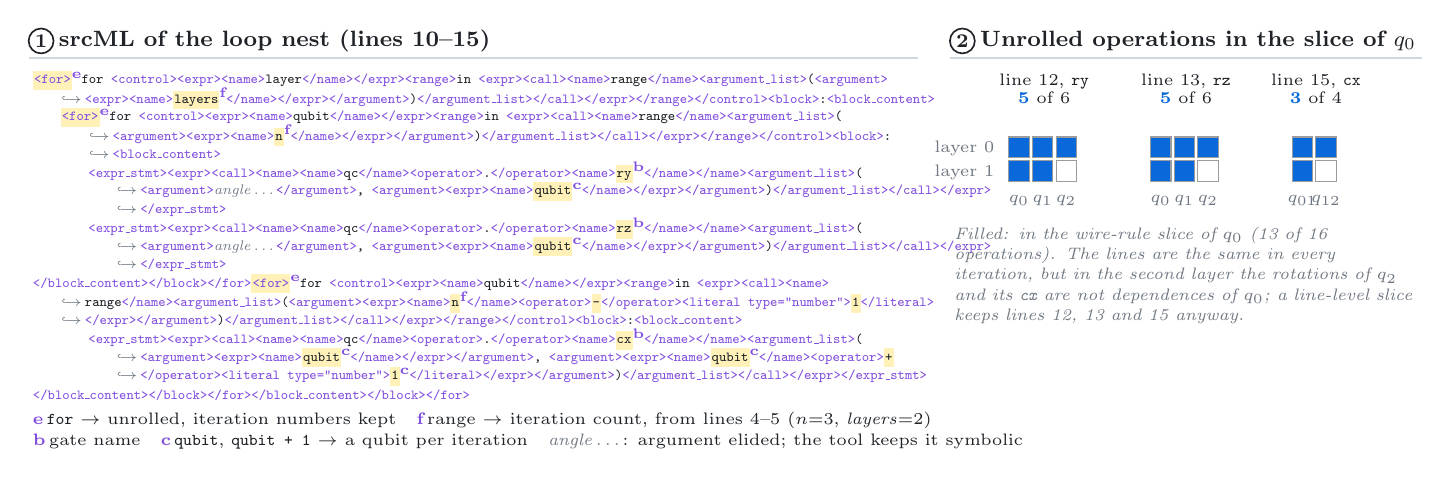
\begin{tikzpicture}

\node[stnum] at (0.16,0.5) {1};
\node[stage] at (0.38,0.5) {srcML of the loop nest (lines 10--15)};
\draw[rule, line width=0.6pt] (0,0.28) -- (11.3,0.28);
\node[xml] at (0.05,0.0) {\hlbox{\textcolor{tree}{<for>}}\hlm{e}\textcolor{ink}{\bfseries for }\textcolor{tree}{<control>}\textcolor{tree}{<expr>}\textcolor{tree}{<name>}\textcolor{ink}{\bfseries layer}\textcolor{tree}{</name>}\textcolor{tree}{</expr>}\textcolor{ink}{\bfseries  }\textcolor{tree}{<range>}\textcolor{ink}{\bfseries in }\textcolor{tree}{<expr>}\textcolor{tree}{<call>}\textcolor{tree}{<name>}\textcolor{ink}{\bfseries range}\textcolor{tree}{</name>}\textcolor{tree}{<argument\_list>}\textcolor{ink}{\bfseries (}\textcolor{tree}{<argument>}};
\node[xml] at (0.40199999999999997,-0.235) {\textcolor{mute}{\rmfamily\fontsize{5}{6}\selectfont$\hookrightarrow$}\,\textcolor{tree}{<expr>}\textcolor{tree}{<name>}\hlbox{\textcolor{ink}{\bfseries layers}}\hlm{f}\textcolor{tree}{</name>}\textcolor{tree}{</expr>}\textcolor{tree}{</argument>}\textcolor{ink}{\bfseries )}\textcolor{tree}{</argument\_list>}\textcolor{tree}{</call>}\textcolor{tree}{</expr>}\textcolor{tree}{</range>}\textcolor{tree}{</control>}\textcolor{tree}{<block>}\textcolor{ink}{\bfseries :}\textcolor{tree}{<block\_content>}};
\node[xml] at (0.40199999999999997,-0.47) {\hlbox{\textcolor{tree}{<for>}}\hlm{e}\textcolor{ink}{\bfseries for }\textcolor{tree}{<control>}\textcolor{tree}{<expr>}\textcolor{tree}{<name>}\textcolor{ink}{\bfseries qubit}\textcolor{tree}{</name>}\textcolor{tree}{</expr>}\textcolor{ink}{\bfseries  }\textcolor{tree}{<range>}\textcolor{ink}{\bfseries in }\textcolor{tree}{<expr>}\textcolor{tree}{<call>}\textcolor{tree}{<name>}\textcolor{ink}{\bfseries range}\textcolor{tree}{</name>}\textcolor{tree}{<argument\_list>}\textcolor{ink}{\bfseries (}};
\node[xml] at (0.754,-0.705) {\textcolor{mute}{\rmfamily\fontsize{5}{6}\selectfont$\hookrightarrow$}\,\textcolor{tree}{<argument>}\textcolor{tree}{<expr>}\textcolor{tree}{<name>}\hlbox{\textcolor{ink}{\bfseries n}}\hlm{f}\textcolor{tree}{</name>}\textcolor{tree}{</expr>}\textcolor{tree}{</argument>}\textcolor{ink}{\bfseries )}\textcolor{tree}{</argument\_list>}\textcolor{tree}{</call>}\textcolor{tree}{</expr>}\textcolor{tree}{</range>}\textcolor{tree}{</control>}\textcolor{tree}{<block>}\textcolor{ink}{\bfseries :}};
\node[xml] at (0.754,-0.94) {\textcolor{mute}{\rmfamily\fontsize{5}{6}\selectfont$\hookrightarrow$}\,\textcolor{tree}{<block\_content>}};
\node[xml] at (0.754,-1.1749999999999998) {\textcolor{tree}{<expr\_stmt>}\textcolor{tree}{<expr>}\textcolor{tree}{<call>}\textcolor{tree}{<name>}\textcolor{tree}{<name>}\textcolor{ink}{\bfseries qc}\textcolor{tree}{</name>}\textcolor{tree}{<operator>}\textcolor{ink}{\bfseries .}\textcolor{tree}{</operator>}\textcolor{tree}{<name>}\hlbox{\textcolor{ink}{\bfseries ry}}\hlm{b}\textcolor{tree}{</name>}\textcolor{tree}{</name>}\textcolor{tree}{<argument\_list>}\textcolor{ink}{\bfseries (}};
\node[xml] at (1.106,-1.41) {\textcolor{mute}{\rmfamily\fontsize{5}{6}\selectfont$\hookrightarrow$}\,\textcolor{tree}{<argument>}\textcolor{mute}{\rmfamily\itshape angle\,\ldots}\textcolor{tree}{</argument>}\textcolor{ink}{\bfseries , }\textcolor{tree}{<argument>}\textcolor{tree}{<expr>}\textcolor{tree}{<name>}\hlbox{\textcolor{ink}{\bfseries qubit}}\hlm{c}\textcolor{tree}{</name>}\textcolor{tree}{</expr>}\textcolor{tree}{</argument>}\textcolor{ink}{\bfseries )}\textcolor{tree}{</argument\_list>}\textcolor{tree}{</call>}\textcolor{tree}{</expr>}};
\node[xml] at (1.106,-1.645) {\textcolor{mute}{\rmfamily\fontsize{5}{6}\selectfont$\hookrightarrow$}\,\textcolor{tree}{</expr\_stmt>}};
\node[xml] at (0.754,-1.88) {\textcolor{tree}{<expr\_stmt>}\textcolor{tree}{<expr>}\textcolor{tree}{<call>}\textcolor{tree}{<name>}\textcolor{tree}{<name>}\textcolor{ink}{\bfseries qc}\textcolor{tree}{</name>}\textcolor{tree}{<operator>}\textcolor{ink}{\bfseries .}\textcolor{tree}{</operator>}\textcolor{tree}{<name>}\hlbox{\textcolor{ink}{\bfseries rz}}\hlm{b}\textcolor{tree}{</name>}\textcolor{tree}{</name>}\textcolor{tree}{<argument\_list>}\textcolor{ink}{\bfseries (}};
\node[xml] at (1.106,-2.1149999999999998) {\textcolor{mute}{\rmfamily\fontsize{5}{6}\selectfont$\hookrightarrow$}\,\textcolor{tree}{<argument>}\textcolor{mute}{\rmfamily\itshape angle\,\ldots}\textcolor{tree}{</argument>}\textcolor{ink}{\bfseries , }\textcolor{tree}{<argument>}\textcolor{tree}{<expr>}\textcolor{tree}{<name>}\hlbox{\textcolor{ink}{\bfseries qubit}}\hlm{c}\textcolor{tree}{</name>}\textcolor{tree}{</expr>}\textcolor{tree}{</argument>}\textcolor{ink}{\bfseries )}\textcolor{tree}{</argument\_list>}\textcolor{tree}{</call>}\textcolor{tree}{</expr>}};
\node[xml] at (1.106,-2.3499999999999996) {\textcolor{mute}{\rmfamily\fontsize{5}{6}\selectfont$\hookrightarrow$}\,\textcolor{tree}{</expr\_stmt>}};
\node[xml] at (0.05,-2.585) {\textcolor{tree}{</block\_content>}\textcolor{tree}{</block>}\textcolor{tree}{</for>}\textcolor{ink}{\bfseries     }\hlbox{\textcolor{tree}{<for>}}\hlm{e}\textcolor{ink}{\bfseries for }\textcolor{tree}{<control>}\textcolor{tree}{<expr>}\textcolor{tree}{<name>}\textcolor{ink}{\bfseries qubit}\textcolor{tree}{</name>}\textcolor{tree}{</expr>}\textcolor{ink}{\bfseries  }\textcolor{tree}{<range>}\textcolor{ink}{\bfseries in }\textcolor{tree}{<expr>}\textcolor{tree}{<call>}\textcolor{tree}{<name>}};
\node[xml] at (0.40199999999999997,-2.82) {\textcolor{mute}{\rmfamily\fontsize{5}{6}\selectfont$\hookrightarrow$}\,\textcolor{ink}{\bfseries range}\textcolor{tree}{</name>}\textcolor{tree}{<argument\_list>}\textcolor{ink}{\bfseries (}\textcolor{tree}{<argument>}\textcolor{tree}{<expr>}\textcolor{tree}{<name>}\hlbox{\textcolor{ink}{\bfseries n}}\hlm{f}\textcolor{tree}{</name>}\textcolor{ink}{\bfseries  }\textcolor{tree}{<operator>}\hlbox{\textcolor{ink}{\bfseries -}}\textcolor{tree}{</operator>}\textcolor{ink}{\bfseries  }\textcolor{tree}{<literal type="number">}\hlbox{\textcolor{ink}{\bfseries 1}}\textcolor{tree}{</literal>}};
\node[xml] at (0.40199999999999997,-3.0549999999999997) {\textcolor{mute}{\rmfamily\fontsize{5}{6}\selectfont$\hookrightarrow$}\,\textcolor{tree}{</expr>}\textcolor{tree}{</argument>}\textcolor{ink}{\bfseries )}\textcolor{tree}{</argument\_list>}\textcolor{tree}{</call>}\textcolor{tree}{</expr>}\textcolor{tree}{</range>}\textcolor{tree}{</control>}\textcolor{tree}{<block>}\textcolor{ink}{\bfseries :}\textcolor{tree}{<block\_content>}};
\node[xml] at (0.754,-3.29) {\textcolor{tree}{<expr\_stmt>}\textcolor{tree}{<expr>}\textcolor{tree}{<call>}\textcolor{tree}{<name>}\textcolor{tree}{<name>}\textcolor{ink}{\bfseries qc}\textcolor{tree}{</name>}\textcolor{tree}{<operator>}\textcolor{ink}{\bfseries .}\textcolor{tree}{</operator>}\textcolor{tree}{<name>}\hlbox{\textcolor{ink}{\bfseries cx}}\hlm{b}\textcolor{tree}{</name>}\textcolor{tree}{</name>}\textcolor{tree}{<argument\_list>}\textcolor{ink}{\bfseries (}};
\node[xml] at (1.106,-3.525) {\textcolor{mute}{\rmfamily\fontsize{5}{6}\selectfont$\hookrightarrow$}\,\textcolor{tree}{<argument>}\textcolor{tree}{<expr>}\textcolor{tree}{<name>}\hlbox{\textcolor{ink}{\bfseries qubit}}\hlm{c}\textcolor{tree}{</name>}\textcolor{tree}{</expr>}\textcolor{tree}{</argument>}\textcolor{ink}{\bfseries , }\textcolor{tree}{<argument>}\textcolor{tree}{<expr>}\textcolor{tree}{<name>}\hlbox{\textcolor{ink}{\bfseries qubit}}\hlm{c}\textcolor{tree}{</name>}\textcolor{ink}{\bfseries  }\textcolor{tree}{<operator>}\hlbox{\textcolor{ink}{\bfseries +}}};
\node[xml] at (1.106,-3.76) {\textcolor{mute}{\rmfamily\fontsize{5}{6}\selectfont$\hookrightarrow$}\,\textcolor{tree}{</operator>}\textcolor{ink}{\bfseries  }\textcolor{tree}{<literal type="number">}\hlbox{\textcolor{ink}{\bfseries 1}}\hlm{c}\textcolor{tree}{</literal>}\textcolor{tree}{</expr>}\textcolor{tree}{</argument>}\textcolor{ink}{\bfseries )}\textcolor{tree}{</argument\_list>}\textcolor{tree}{</call>}\textcolor{tree}{</expr>}\textcolor{tree}{</expr\_stmt>}};
\node[xml] at (0.05,-3.9949999999999997) {\textcolor{tree}{</block\_content>}\textcolor{tree}{</block>}\textcolor{tree}{</for>}\textcolor{tree}{</block\_content>}\textcolor{tree}{</block>}\textcolor{tree}{</for>}};
\node[anchor=north west, align=left, font=\fontsize{6.2}{7.6}\selectfont, text=ink, inner sep=0pt] at (0.05,-4.21) {\hl{e}\,\texttt{for} $\to$ unrolled, iteration numbers kept\quad \hl{f}\,range $\to$ iteration count, from lines 4--5 ($n{=}3$, $\mathit{layers}{=}2$)\\\hl{b}\,gate name\quad \hl{c}\,\texttt{qubit}, \texttt{qubit + 1} $\to$ a qubit per iteration\quad \textcolor{mute}{\itshape angle\,\ldots}: argument elided; the tool keeps it symbolic};
\node[stnum] at (11.860000000000001,0.5) {2};
\node[stage] at (12.080000000000002,0.5) {Unrolled operations in the slice of $q_0$};
\draw[rule, line width=0.6pt] (11.700000000000001,0.28) -- (17.700000000000003,0.28);
\node[font=\fontsize{6.3}{7.4}\selectfont, text=ink, anchor=south, align=center] at (12.9,-0.42) {line 12, \texttt{ry}\\[-1pt]\textcolor{wire}{\bfseries 5} of 6};
\node[font=\fontsize{5.8}{6.5}\selectfont, text=mute, anchor=east] at (12.39,-0.87) {layer 0};
\draw[draw=ink!45, line width=0.4pt, fill=wire] (12.450000000000001,-0.72) rectangle ++(0.26,-0.26);
\draw[draw=ink!45, line width=0.4pt, fill=wire] (12.750000000000002,-0.72) rectangle ++(0.26,-0.26);
\draw[draw=ink!45, line width=0.4pt, fill=wire] (13.05,-0.72) rectangle ++(0.26,-0.26);
\node[font=\fontsize{5.8}{6.5}\selectfont, text=mute, anchor=east] at (12.39,-1.17) {layer 1};
\draw[draw=ink!45, line width=0.4pt, fill=wire] (12.450000000000001,-1.02) rectangle ++(0.26,-0.26);
\draw[draw=ink!45, line width=0.4pt, fill=wire] (12.750000000000002,-1.02) rectangle ++(0.26,-0.26);
\draw[draw=ink!45, line width=0.4pt, fill=white] (13.05,-1.02) rectangle ++(0.26,-0.26);
\node[font=\fontsize{5.6}{6}\selectfont, text=mute, anchor=north] at (12.580000000000002,-1.3399999999999999) {$q_{0}$};
\node[font=\fontsize{5.6}{6}\selectfont, text=mute, anchor=north] at (12.880000000000003,-1.3399999999999999) {$q_{1}$};
\node[font=\fontsize{5.6}{6}\selectfont, text=mute, anchor=north] at (13.180000000000001,-1.3399999999999999) {$q_{2}$};
\node[font=\fontsize{6.3}{7.4}\selectfont, text=ink, anchor=south, align=center] at (14.700000000000001,-0.42) {line 13, \texttt{rz}\\[-1pt]\textcolor{wire}{\bfseries 5} of 6};
\draw[draw=ink!45, line width=0.4pt, fill=wire] (14.250000000000002,-0.72) rectangle ++(0.26,-0.26);
\draw[draw=ink!45, line width=0.4pt, fill=wire] (14.550000000000002,-0.72) rectangle ++(0.26,-0.26);
\draw[draw=ink!45, line width=0.4pt, fill=wire] (14.850000000000001,-0.72) rectangle ++(0.26,-0.26);
\draw[draw=ink!45, line width=0.4pt, fill=wire] (14.250000000000002,-1.02) rectangle ++(0.26,-0.26);
\draw[draw=ink!45, line width=0.4pt, fill=wire] (14.550000000000002,-1.02) rectangle ++(0.26,-0.26);
\draw[draw=ink!45, line width=0.4pt, fill=white] (14.850000000000001,-1.02) rectangle ++(0.26,-0.26);
\node[font=\fontsize{5.6}{6}\selectfont, text=mute, anchor=north] at (14.380000000000003,-1.3399999999999999) {$q_{0}$};
\node[font=\fontsize{5.6}{6}\selectfont, text=mute, anchor=north] at (14.680000000000003,-1.3399999999999999) {$q_{1}$};
\node[font=\fontsize{5.6}{6}\selectfont, text=mute, anchor=north] at (14.980000000000002,-1.3399999999999999) {$q_{2}$};
\node[font=\fontsize{6.3}{7.4}\selectfont, text=ink, anchor=south, align=center] at (16.35,-0.42) {line 15, \texttt{cx}\\[-1pt]\textcolor{wire}{\bfseries 3} of 4};
\draw[draw=ink!45, line width=0.4pt, fill=wire] (16.05,-0.72) rectangle ++(0.26,-0.26);
\draw[draw=ink!45, line width=0.4pt, fill=wire] (16.35,-0.72) rectangle ++(0.26,-0.26);
\draw[draw=ink!45, line width=0.4pt, fill=wire] (16.05,-1.02) rectangle ++(0.26,-0.26);
\draw[draw=ink!45, line width=0.4pt, fill=white] (16.35,-1.02) rectangle ++(0.26,-0.26);
\node[font=\fontsize{5.6}{6}\selectfont, text=mute, anchor=north] at (16.18,-1.3399999999999999) {$q_{01}$};
\node[font=\fontsize{5.6}{6}\selectfont, text=mute, anchor=north] at (16.48,-1.3399999999999999) {$q_{12}$};
\node[note, anchor=north west, align=left, text width=5.9cm] at (11.750000000000002,-1.85) {Filled: in the wire-rule slice of $q_0$ (13 of 16 operations). The lines are the same in every iteration, but in the second layer the rotations of $q_2$ and its \texttt{cx} are not dependences of $q_0$; a line-level slice keeps lines 12, 13 and 15 anyway.};
\end{tikzpicture}
\end{document}
